\section{Main System Components}
	


	\subsection{Photodiode}
	
		Photodiode will be used as a detector in a reflective configuration, wherein light is projected from one end using LEDs and photodiode is detecting light at the opposite end converting it to current. This current would be proportional to LEDs brightness.
		
		
		\begin{figure}[ht!]
			\centering
			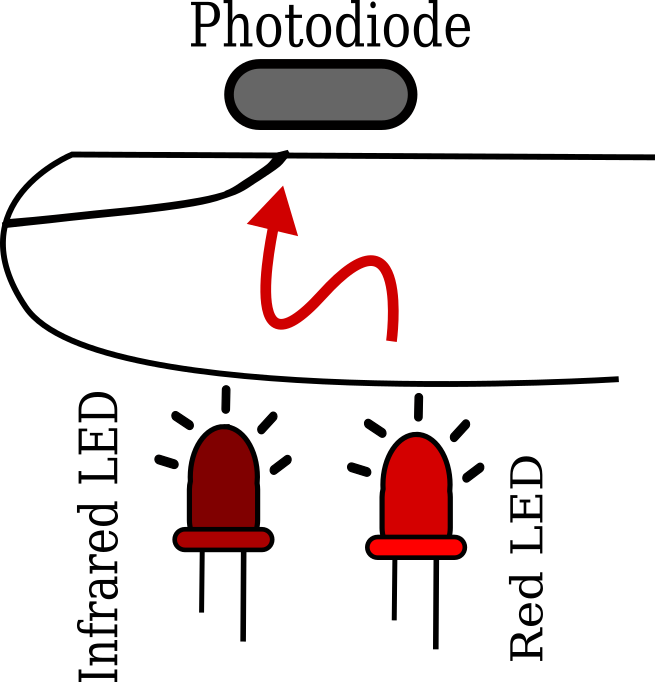
\includegraphics[width=0.3\textwidth]{images/finger_setup_en.png}
			\caption{Reflective finger setup}
		\end{figure}

		Photodiode needs to be sensitive in both red (700nm) and infrared (900nm) regions. QSB34CGR was used in this design which can work in both regions as seen in the sensitivity graph from part's datasheet.
	
		\begin{figure}[ht!]
			\centering
			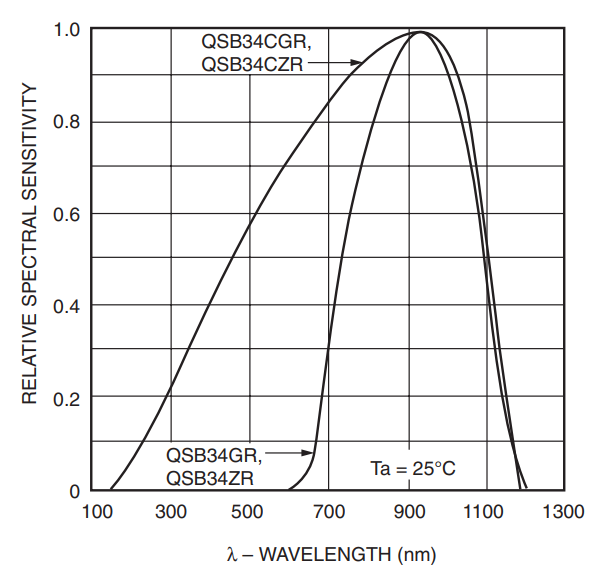
\includegraphics[width=0.6\textwidth]{../common/QSBCGR.png}
			\caption{QSB34CGR sensitivity spectrum}
		\end{figure}
	
	\pagebreak
	
	\subsection{Microcontroller}
	
		Microcontroller($\mu$C) is responsible for the algorithm in calculating the SpO\textsubscript{2} by reading the red and ir amplified channels via ADC. Also it performs the following tasks:
		
		\begin{itemize}
			\item Interfaces with an OLED 128x64 display to show the calculated  SpO\textsubscript{2} and heart beat.
			
			\item Interfaces with DACs.
		\end{itemize}
		
		Atmega4808 is used in this design.
	
	\subsection{Dual DAC}
	
		Dual digital to analog converter - MCP47FEB02A0 was used in design.
		
		\begin{itemize}
			
			\item DAC1 is required in LED driver stage so that $\mu$C can instruct the DAC to generate a required control voltage to set led current.
			
			\item DAC2 provides an input to the difference amplifier stage for DC removal from signals.
		
		\end{itemize}
		
	\subsection{Leds}
		It is important to select good leds for illumination, following factors ensure good signal response:
		
		\begin{itemize}
			\item Narrow view angle for less dispersion and deeper penetration into skin.
			\item Rectangular package in clear lens so that finger can rest comfortably.
			\item High radiant power.
		\end{itemize}
	
		I didn't get new leds and worked with generic 3mm/5mm ir led in circular clear package and a red led in diffused package. This caused the R ratio to not be correct. As a healthy individual, i was getting readings of R to be around 0.6 while it should be around 0.4. So I had to use a scaling factor to adjust the algorithm. A comment has been added in the program code regarding this. 
		
		A suitable choice can be Vishay Semiconductor's VSMD66694.
	
		  
	